\section{Durchführung}

    Für die folgenden Messungen ist ein Lock-In-Verstärker,
    welcher in Abbildung \ref{fig:verstärker} dargestellt ist,
    sowie ein Speicheroszilloskop gegeben.
    \begin{figure}[H]
        \centering
        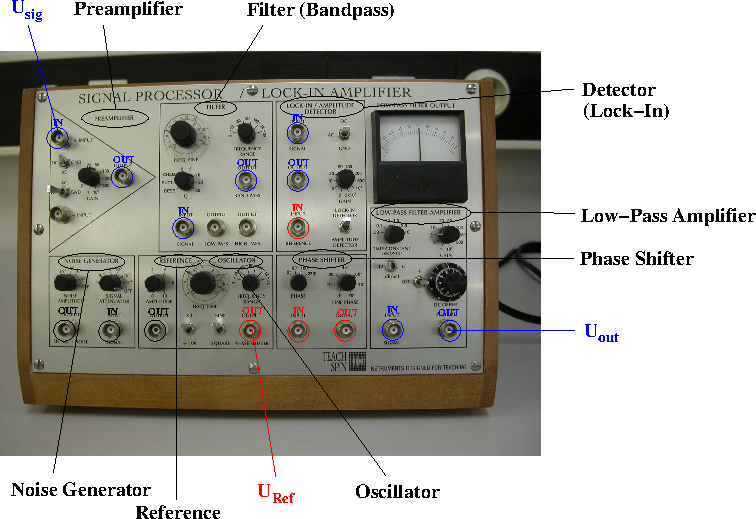
\includegraphics[scale=1]{content/img/Abb_3.pdf}
        \caption{Aufbau des Lock-In-Verstärkers.}
        \label{fig:verstärker}
    \end{figure}
    Der Lock-In-Verstärker beinhaltet neben dem Bandpass,
    dem Phasenverschieber und dem Tiefpass ebenfalls einen Vorverstärker,
    einen Funktions- und Rauschgenerator und einen Tiefpass-Verstärker,
    sowie ein Amplituden/Lock-In-Detektor.\\
    \\
    Für die ersten beiden Messungen wird der Lock-In-Verstärker nach dem folgenden Schaltbild aufgebaut.
    \begin{figure}[H]
        \centering
        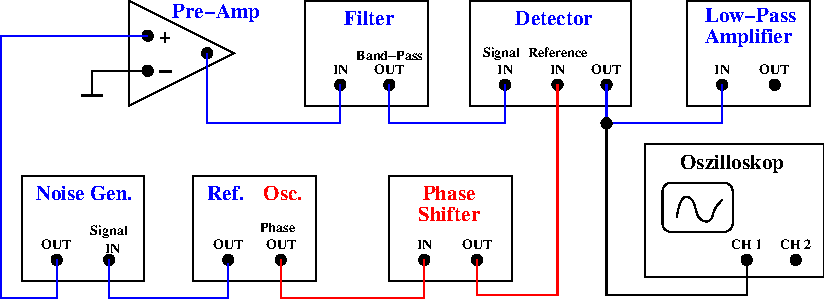
\includegraphics[scale=1]{content/img/Abb_4.pdf}
        \caption{Schaltbild zur Messung des Ausgangssignals in Abhängigkeit von der Phasenverschiebung.}
        \label{fig:schaltung1}
    \end{figure}
    Bei der ersten Messung wird ohne ein zusätzliches Rauschen gearbeitet,
    sodass der Noise-Generator in der Schaltung überbrückt wird.
    Das sinusförmige Eingangssignal $U_\text{Sig}$ wird auf eine Frequenz von $\SI{1}{\kilo\hertz}$ eingestellt,
    wobei hier darauf geachtet werden muss,
    dass die gleiche Frequenz für die Referenzspannung $U_\text{Ref}$,
    welche ebenfalls sinusförmig ist,
    eingestellt werden muss.
    Es wird eine Verstärkung von $\SI{10}{\milli\volt}$ eingestellt.
    Nun wird die Ausgangsspannung $U_\text{Out}$ in Abhängigkeit von der Phasenverschiebung $\phi$ gemessen.
    Es werden etwa zehn Messwerte aufgenommen und deren Bilder mit dem Speicheroszilloskop gespeichert.
    Die Ausgangsspannung kann mit den berechneten Werten aus der Gleichung \eqref{eqn:ausgangsspannung_phase} verglichen werden.\\%(?)
    Für die zweite Messung wird nun ein Rauschsignal auf dem Noise-Generator hinzugefügt,
    welcher dazu wieder in die Schaltung in Abbildung \ref{fig:schaltung1} integriert werden muss.
    Das Rauschsignal wird auf die Größenordnung der Signalspannung,
    in diesem Fall also $\SI{e-2}{\volt}$,
    eingestellt und das Verfahren der ersten Messung wird wiederholt.\\
    \\
    Anschließend soll der Lock-In-Verstärker in Verbindung mit einem Photodetektor untersucht werden.
    Dazu wird die folgende Schaltung verwendet.
    \begin{figure}[H]
        \centering
        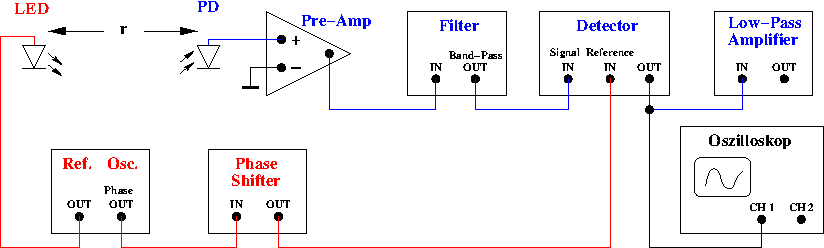
\includegraphics[scale=1]{content/img/Abb_5.pdf}
        \caption{Schaltbild zur Messung der Ausgangsspannung eines Photodetektors.}
        \label{fig:schaltung2}
    \end{figure}
    Die Leuchtdiode,
    welche mit einer Frequenz von $\SI{500}{\hertz}$ bei einer Rechteckspannung %von $\SI{10}{\milli\volt}$ %TODO
    blinkt,
    ist auf eine Photodiode gerichtet.
    Es wird die Spannung an der Photodiode in Abhängigkeit des Abstandes zwischen Leuchtdiode und Photodiode gemessen.
    Dazu sind beide Dioden auf einer skallierten Messschiene befestigt,
    wobei der minimale Abstand zwischen den Dioden $\SI{5}{\centi\meter}$ beträgt.
    Die Leuchtdiode wird nun immer weiter von der Photodiode weg geschoben und gleichzeitig wird die registrierte Spannung gemessen.

        